\documentclass[notes,11pt, aspectratio=169]{beamer}

\usepackage{pgfpages}
% These slides also contain speaker notes. You can print just the slides,
% just the notes, or both, depending on the setting below. Comment out the want
% you want.
\setbeameroption{hide notes} % Only slide
%\setbeameroption{show only notes} % Only notes
%\setbeameroption{show notes on second screen=right} % Both

\usepackage{helvet}
\usepackage[default]{lato}
\usepackage{array}


\usepackage{tikz}
\usepackage{verbatim}
\setbeamertemplate{note page}{\pagecolor{yellow!5}\insertnote}
\usetikzlibrary{positioning}
\usetikzlibrary{snakes}
\usetikzlibrary{calc}
\usetikzlibrary{arrows}
\usetikzlibrary{decorations.markings}
\usetikzlibrary{shapes.misc}
\usetikzlibrary{matrix,shapes,arrows,fit,tikzmark}
\usepackage{amsmath}
\usepackage{mathpazo}
\usepackage{hyperref}
\usepackage{lipsum}
\usepackage{multimedia}
\usepackage{graphicx}
\usepackage{multirow}
\usepackage{graphicx}
\usepackage{dcolumn}
\usepackage{bbm}
\newcolumntype{d}[0]{D{.}{.}{5}}

\usepackage{changepage}
\usepackage{appendixnumberbeamer}
\newcommand{\beginbackup}{
   \newcounter{framenumbervorappendix}
   \setcounter{framenumbervorappendix}{\value{framenumber}}
   \setbeamertemplate{footline}
   {
     \leavevmode%
     \hline
     box{%
       \begin{beamercolorbox}[wd=\paperwidth,ht=2.25ex,dp=1ex,right]{footlinecolor}%
%         \insertframenumber  \hspace*{2ex} 
       \end{beamercolorbox}}%
     \vskip0pt%
   }
 }
\newcommand{\backupend}{
   \addtocounter{framenumbervorappendix}{-\value{framenumber}}
   \addtocounter{framenumber}{\value{framenumbervorappendix}} 
}


\usepackage{graphicx}
\usepackage[space]{grffile}
\usepackage{booktabs}

% These are my colors -- there are many like them, but these ones are mine.
\definecolor{blue}{RGB}{0,114,178}
\definecolor{red}{RGB}{213,94,0}
\definecolor{yellow}{RGB}{240,228,66}
\definecolor{green}{RGB}{0,158,115}

\hypersetup{
  colorlinks=false,
  linkbordercolor = {white},
  linkcolor = {blue}
}


%% I use a beige off white for my background
\definecolor{MyBackground}{RGB}{255,253,218}

%% Uncomment this if you want to change the background color to something else
%\setbeamercolor{background canvas}{bg=MyBackground}

%% Change the bg color to adjust your transition slide background color!
\newenvironment{transitionframe}{
  \setbeamercolor{background canvas}{bg=yellow}
  \begin{frame}}{
    \end{frame}
}

\setbeamercolor{frametitle}{fg=blue}
\setbeamercolor{title}{fg=black}
\setbeamertemplate{footline}[frame number]
\setbeamertemplate{navigation symbols}{} 
\setbeamertemplate{itemize items}{-}
\setbeamercolor{itemize item}{fg=blue}
\setbeamercolor{itemize subitem}{fg=blue}
\setbeamercolor{enumerate item}{fg=blue}
\setbeamercolor{enumerate subitem}{fg=blue}
\setbeamercolor{button}{bg=MyBackground,fg=blue,}



% If you like road maps, rather than having clutter at the top, have a roadmap show up at the end of each section 
% (and after your introduction)
% Uncomment this is if you want the roadmap!
% \AtBeginSection[]
% {
%    \begin{frame}
%        \frametitle{Roadmap of Talk}
%        \tableofcontents[currentsection]
%    \end{frame}
% }
\setbeamercolor{section in toc}{fg=blue}
\setbeamercolor{subsection in toc}{fg=red}
\setbeamersize{text margin left=1em,text margin right=1em} 

\newenvironment{wideitemize}{\itemize\addtolength{\itemsep}{10pt}}{\enditemize}

\usepackage{environ}
\NewEnviron{videoframe}[1]{
  \begin{frame}
    \vspace{-8pt}
    \begin{columns}[onlytextwidth, T] % align columns
      \begin{column}{.58\textwidth}
        \begin{minipage}[t][\textheight][t]
          {\dimexpr\textwidth}
          \vspace{8pt}
          \hspace{4pt} {\Large \sc \textcolor{blue}{#1}}
          \vspace{8pt}
          
          \BODY
        \end{minipage}
      \end{column}%
      \hfill%
      \begin{column}{.42\textwidth}
        \colorbox{green!20}{\begin{minipage}[t][1.2\textheight][t]
            {\dimexpr\textwidth}
            Face goes here
          \end{minipage}}
      \end{column}%
    \end{columns}
  \end{frame}
}

% Add code blocks
\usepackage{listings}
\lstset{
basicstyle=\ttfamily\tiny,
numbers=left,
numberstyle=\tiny,
frame=single,
breaklines=true,
commentstyle=\color{green!60!black},
keywordstyle=\color{blue},
stringstyle=\color{red},
showstringspaces=false
}

\title[]{\textcolor{blue}{Numerical Integration}}
\author[CTM]{Charlie Murry}
% \institute[FRBNY]{\small{\begin{tabular}{c c c}
% Charlie Murry && \\
% U Michigan &&  \\ \\

% Author C && Author D   \\
% \multicolumn{3}{c}{Somewhere Fancy} \\
% \end{tabular}}}

\date{January 2025}

\begin{document}

\begin{frame}
\titlepage
\end{frame}

\begin{frame}{Numerical Differentiation and Integration}
\begin{wideitemize}
\item General form: $\int_I f(x)w(x)dx \approx \sum_{i=0}^n w_i f(x_i)$
\item Components:
    \begin{itemize}
    \item Nodes ($x_i$)
    \item Weights ($w_i$)
    \end{itemize}
\end{wideitemize}
\end{frame}

\begin{frame}{Midpoint Rule}
\begin{wideitemize}
\item Approximates integral using rectangles
\item Node at midpoint of each interval
\item Simple but less accurate than other methods
\end{wideitemize}

\begin{center}
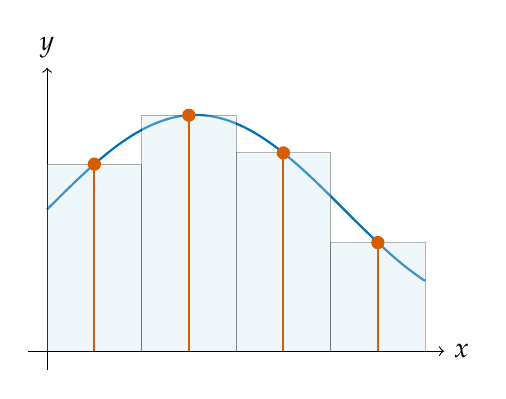
\begin{tikzpicture}[scale=1.2]
    % Define the function curve
    \draw[thick, blue, domain=0:4, samples=100] plot (\x, {1.5 + sin(\x r)});
    
    % Draw axes
    \draw[->] (-0.2,0) -- (4.2,0) node[right] {$x$};
    \draw[->] (0,-0.2) -- (0,3) node[above] {$y$};
    
    % Draw rectangles
    \foreach \i in {0,1,2,3} {
        \draw[fill=blue!20, opacity=0.3] (\i,0) rectangle ++ (1,{1.5 + sin((\i + 0.5) r)});
        \draw[red, thick] (\i + 0.5,0) -- (\i + 0.5,{1.5 + sin((\i + 0.5) r)});
        \fill[red] (\i + 0.5,{1.5 + sin((\i + 0.5) r)}) circle (2pt);
    }
\end{tikzpicture}
\end{center}
\end{frame}

\begin{frame}{Trapezoidal Rule}
\begin{wideitemize}
\item Uses linear approximation between points
\item Formula: $\int_a^b f(x)dx \approx \frac{b-a}{2n}[f(x_0) + 2f(x_1) + ... + f(x_{n+1})]$
\item More accurate than midpoint rule
\end{wideitemize}

\begin{center}
    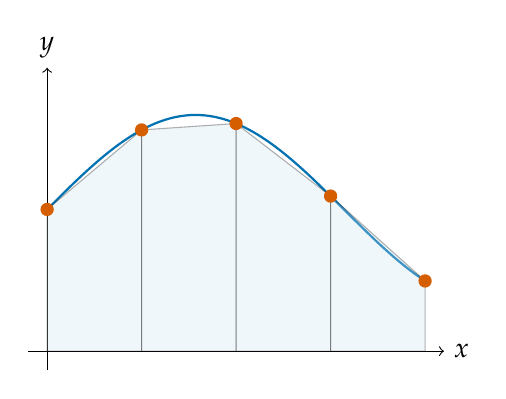
\begin{tikzpicture}[scale=1.2]
    % Define the function curve
    \draw[thick, blue, domain=0:4, samples=100] plot (\x, {1.5 + sin(\x r)});

    % Draw axes
\draw[->] (-0.2,0) -- (4.2,0) node[right] {$x$};
\draw[->] (0,-0.2) -- (0,3) node[above] {$y$};

% Draw trapezoids
\foreach \i in {0,1,2,3} {
    \draw[fill=blue!20, opacity=0.3] (\i,0) -- 
        (\i,{1.5 + sin(\i r)}) -- 
        (\i + 1,{1.5 + sin((\i + 1) r)}) -- 
        (\i + 1,0) -- cycle;
    \fill[red] (\i,{1.5 + sin(\i r)}) circle (2pt);
}
\fill[red] (4,{1.5 + sin(4 r)}) circle (2pt);

\end{tikzpicture}
\end{center}
\end{frame}


\begin{frame}{Simpson's Rule}
    \begin{itemize}
    \item Uses parabolic approximation
    \item Formula: $\int_a^b f(x)dx = \frac{h}{3}[f(a) + 4f(\frac{a+b}{2}) + f(b)]$
    \item where $h=\frac{b-a}{n}$ and $n=2$ step size (three points). 
    \item More generally: nodes are evenly spaced: $x_i = a + ih$
    \item Weights:
    \begin{itemize}
    \item $w_0 = w_n = \frac{h}{3}$
    \item $w_i = \frac{4h}{3}$ for even i
    \item $w_i = \frac{2h}{3}$ for odd i
    \end{itemize}
    \end{itemize}

    \begin{center}

        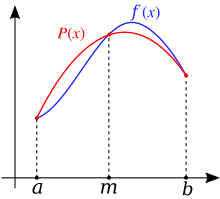
\includegraphics[scale=0.45]{Simpsons_method_illustration.svg.png}
        % \includegraphics[width=0.48\textwidth]{Simpsonsrule2.gif}

    \end{center}
\end{frame}


\begin{frame}{Monte Carlo Integration}
\begin{wideitemize}
    \item Tecnique using (psuedo-)randomly drawn nodes, equally weighted.
\item Relies on the Strong Law of Large Numbers (SLLN).
\begin{quote}
    Sample average converges almost surely to the expected value.
\end{quote}
    \[ \lim_{n\to\infty} \frac{1}{n}\sum_{i=1}^n f(x_i) = E[f(\tilde{X})] \]
\item Nodes: $x_i \rightarrow$ draw from uniform on the computer.
\item Weights: $w_i = \frac{1}{n}$
\end{wideitemize}
\end{frame}

\begin{frame}[fragile]{Simple Julia Script}
        \begin{lstlisting}
            using Statistics

            function mc_integral(f, a, b, n)
                # Generate random points in interval [a,b]
                x = a .+ (b-a) * rand(n)
                
                # Compute function values and scale by interval width
                y = f.(x) * (b-a)
                
                # Return mean and standard error
                return mean(y), std(y)/sqrt(n)
            end
            
            # Test with f(x) = x^2 on [0,1]
            f(x) = x^2
            n = 100000
            result, error = mc_integral(f, 0, 1, n)
            
            println("Integral of x^2 from 0 to 1:")
            println("Monte Carlo: $result ± $error")
            println("Exact: $(1/3)")
        \end{lstlisting}
\end{frame}


\begin{frame}{Quasi-Monte Carlo Methods}
\begin{wideitemize}
    \item Having truley random numbers may waste guesses. 
    \item We can choose nodes that are ``low-discrepency''
\item Improvements over standard Monte Carlo:
    \begin{itemize}
    \item Halton/Sobol sequences for better distribution.
    \item Antithetic acceleration: if using $x_1$, also use $-x_1$.
    \end{itemize}
\item More systematic coverage of integration domain.
\end{wideitemize}
\end{frame}

\begin{frame}{Gaussian Quadrature}
\begin{wideitemize}
\item Nodes and weights chosen "efficiently."
\item Fewwst nodes possible to achieve exact approximation for polynomials. 
\item Even though you may not be dealing with a polynomial, this type of result can be useful in having confidence in your result.
\item Choose $x_i$ and $w_i$ so that aprox is exact with $n$ nodes if $f$ is $P_{2n-1}$
\item Example: Match $2n$ moments of weight function $g(x)$
% \item Systems of equations:
%     \[ \int_a^b x^k g(x)dx = \sum_{i=1}^n w_i x_i^k, \quad k = 0...2n-1 \]
\end{wideitemize}
\end{frame}

\begin{frame}{Gaussian Quadrature Example}
Example: Match $2n$ moments of weight function $g(x)$\\
% For N(0,1) distribution:
Systems of $2n$ equations:
    \[ \int_a^b x^k g(x)dx = \sum_{i=1}^n w_i x_i^k, \quad k = 0...2n-1 \]
    If $g(x)$ is a density, then the $k$ equations are the $k$ uncentered moments of a cont. random variable. 
\end{frame}
\begin{frame}
    If $x\sim N(0,1)$ and $\phi(x)$ is the pdf (weights)\\[1em] 
    Then the first six moments are
% \begin{itemize}
% \item Match first 6 moments of normal distribution
% \item System of equations:
    \begin{align*}
    E(X^0) &= 1 = \sum_{i=1}^3 w_i \\
    E(X^1) &= 0 = \sum_{i=1}^3 w_i x_i \\
    E(X^{5}) &= 0 = \sum_{i=1}^3 w_i x_i^{5}
    \end{align*}
    Solve this system of six equations and six unknowns.
\begin{tabular}{cc}
\hline
$x_i$ & $w_i$ \\
\hline
-1.732 & 0.166 \\
0 & 0.667 \\
1.732 & 0.166 \\
\hline
\end{tabular}    
\end{frame}

\begin{frame}
If you want to find 
$$Var(X) = E(X^2) = \int x^2 \phi(x)dx$$

Then now we know. 
$$\int x^2 \phi(x)dx = \sum_{i=1}^3 w_i x_i = (-1.732)^2(0.166) + (0)^2(0.667) + (1.732)^2(0.166)$$

\vspace{1em}
What is the big deal? 
\begin{wideitemize}
    \item For certain weight functions, people have worked out exactly which nodes and wights you should use if you want $n$ nodes. 
    \item In the case above, we were approximating the integrals of polynomials so we could get it exact. 
    \item In your work, you probably won't have polynomials, but you can still use these $x,n$ to get a high level of precision.
\end{wideitemize}

\end{frame}

% \end{itemize}

% \begin{table}
% \begin{tabular}{cc}
% \hline
% $x_i$ & $w_i$ \\
% \hline
% -1.732 & 0.166 \\
% 0 & 0.667 \\
% 1.732 & 0.166 \\
% \hline
% \end{tabular}
% \end{table}
% \end{frame}

\end{document}